\chapter{Arquitetura e Modelagem do Sistema}

Este capítulo apresenta a arquitetura e modelagem do sistema de registro de ponto eletrônico desenvolvido, detalhando a estrutura organizacional do \textit{software}, as tecnologias empregadas, os padrões arquiteturais adotados e o modelo de dados implementado. O sistema foi concebido seguindo uma arquitetura distribuída, com separação clara entre \textit{frontend} e \textit{backend}, permitindo escalabilidade, manutenibilidade e flexibilidade na evolução da aplicação.

\section{Visão Geral da Arquitetura}

O sistema de registro de ponto eletrônico foi desenvolvido utilizando uma arquitetura em três camadas (3-tier), separando claramente as responsabilidades entre apresentação, lógica de negócio e persistência de dados. Esta abordagem segue os princípios da arquitetura SOA (\textit{Service-Oriented Architecture}) e REST (\textit{Representational State Transfer}), promovendo a interoperabilidade e facilitando a integração com sistemas externos.

A Figura~\ref{fig:arquitetura-geral} apresenta a visão geral da arquitetura do sistema, destacando os principais componentes e suas interações.

\begin{figure}[htbp]
    \centering
    \begin{tikzpicture}[
            node distance=1.5cm,
            box/.style={rectangle, draw, fill=blue!10, text width=3cm, text centered, minimum height=1.2cm},
            api/.style={rectangle, draw, fill=green!10, text width=2.5cm, text centered, minimum height=1cm},
            db/.style={cylinder, draw, fill=yellow!10, text width=2cm, text centered, minimum height=1.5cm, aspect=0.25},
            external/.style={rectangle, draw, fill=red!10, text width=2.5cm, text centered, minimum height=1cm},
            arrow/.style={->, thick}
        ]

        % Frontend Layer
        \node[box] (client) at (0,6) {Cliente Web\\(Next.js 15)};
        \node[box] (auth) at (0,4) {Autenticação\\(NextAuth.js)};

        % API Gateway
        \node[api] (gateway) at (5,5) {API Gateway\\(NestJS)};

        % Backend Services
        \node[api] (auth-service) at (3,2.5) {Auth Service};
        \node[api] (user-service) at (7,2.5) {User Service};
        \node[api] (company-service) at (3,0.5) {Company Service};
        \node[api] (point-service) at (7,0.5) {Point Service};

        % Database
        \node[db] (database) at (11,3) {PostgreSQL\\Database};

        % External Services
        \node[external] (maps) at (2,8) {Google Maps\\API};
        \node[external] (geolocation) at (8,8) {Geolocation\\Services};

        % Connections
        \draw[arrow] (client) -- (gateway) node[midway, above] {HTTPS/REST};
        \draw[arrow] (auth) -- (gateway);
        \draw[arrow] (gateway) -- (auth-service);
        \draw[arrow] (gateway) -- (user-service);
        \draw[arrow] (gateway) -- (company-service);
        \draw[arrow] (gateway) -- (point-service);
        \draw[arrow] (auth-service) -- (database);
        \draw[arrow] (user-service) -- (database);
        \draw[arrow] (company-service) -- (database);
        \draw[arrow] (point-service) -- (database);
        \draw[arrow] (client) -- (maps);
        \draw[arrow] (client) -- (geolocation);

    \end{tikzpicture}
    \caption{Arquitetura geral do sistema de registro de ponto}
    \label{fig:arquitetura-geral}
\end{figure}

A arquitetura adotada proporciona as seguintes vantagens:

\begin{itemize}
    \item \textbf{Separação de Responsabilidades}: Cada camada possui responsabilidades bem definidas, facilitando a manutenção e evolução do sistema;
    \item \textbf{Escalabilidade}: A arquitetura permite escalar horizontalmente cada componente de forma independente;
    \item \textbf{Testabilidade}: A separação em camadas facilita a implementação de testes unitários e de integração;
    \item \textbf{Reutilização}: Os serviços do \textit{backend} podem ser consumidos por diferentes clientes;
    \item \textbf{Segurança}: A centralização da lógica de autenticação e autorização no \textit{backend} garante maior segurança.
\end{itemize}

\section{Modelagem de Dados}

O modelo de dados foi projetado seguindo os princípios da normalização de banco de dados e os padrões do Domain-Driven Design (DDD). O sistema utiliza PostgreSQL como sistema de gerenciamento de banco de dados, aproveitando suas características de robustez, conformidade com ACID e suporte a tipos de dados complexos.

A Figura~\ref{fig:modelo-entidades} apresenta o diagrama de classes UML resumido do modelo de dados, destacando as principais entidades, seus atributos, métodos e relacionamentos.

\begin{figure}[htbp]
    \centering
    \resizebox{0.75\textwidth}{!}{%
        \begin{tikzpicture}[scale=0.3,every node/.style={transform shape}]

            % Organização hierárquica com espaçamento ampliado

            % Nível 1: Entidade principal
            \umlclass[x=8, y=20, width=2cm]{Empresa}{
                + id: UUID \\
                + nome: String \\
                + cnpj: String \\
                + email: String \\
                + telefone: String \\
                + endereco: Text \\
                + latitude: Decimal \\
                + longitude: Decimal \\
                + raioPermitido: Integer \\
                + toleranciaEntrada: Integer \\
                + toleranciaSaida: Integer \\
                + exigirJustificativaForaRaio: Boolean \\
                + createdAt: Date \\
                + updatedAt: Date
            }{
            }

            % Nível 2: Entidades dependentes da empresa  
            \umlclass[x=0, y=14, width=1.6cm]{Departamento}{
                + id: UUID \\
                + nome: String \\
                + descricao: Text \\
                + empresaId: UUID \\
                + createdAt: Date \\
                + updatedAt: Date
            }{
            }

            \umlclass[x=8, y=10, width=2cm]{Usuario}{
                + id: UUID \\
                + nome: String \\
                + email: String \\
                + password: String \\
                + telefone: String \\
                + photoUrl: String \\
                + cpf: String \\
                + papel: UserRole \\
                + status: UserStatus \\
                + empresaId: UUID \\
                + createdAt: Date \\
                + updatedAt: Date
            }{
            }

            \umlclass[x=16, y=14, width=2cm]{HorarioFuncionario}{
                + id: UUID \\
                + diaSemana: Integer \\
                + ativo: Boolean \\
                + horarioInicio: Time \\
                + horarioFim: Time \\
                + temIntervalo: Boolean \\
                + intervaloInicio: Time \\
                + intervaloFim: Time \\
                + usuarioId: UUID \\
                + createdAt: Date \\
                + updatedAt: Date
            }{
            }

            % Nível 3: Entidades específicas
            \umlclass[x=0, y=7, width=1.6cm]{Cargo}{
                + id: UUID \\
                + nome: String \\
                + descricao: Text \\
                + baseSalarial: Decimal \\
                + departamentoId: UUID \\
                + createdAt: Date \\
                + updatedAt: Date
            }{
            }

            \umlclass[x=8, y=0, width=2cm]{InformacoesTrabalhistas}{
                + id: UUID \\
                + usuarioId: UUID \\
                + cargoId: UUID \\
                + departamentoId: UUID \\
                + dataAdmissao: Date \\
                + inicioRegistros: Date \\
                + cargaHorariaSemanal: Decimal \\
                + salario: Decimal \\
                + createdAt: Date \\
                + updatedAt: Date
            }{
            }

            % Nível 4: Entidades operacionais
            \umlclass[x=-2, y=0, width=2cm]{RegistroPonto}{
                + id: UUID \\
                + usuarioId: UUID \\
                + tipo: TipoRegistro \\
                + status: StatusRegistro \\
                + dataHora: DateTime \\
                + latitude: Decimal \\
                + longitude: Decimal \\
                + dentroDoRaio: Boolean \\
                + observacoes: Text \\
                + temJustificativaPendente: Boolean \\
                + createdAt: Date \\
                + updatedAt: Date
            }{
            }

            \umlclass[x=17, y=2, width=2cm]{Justificativa}{
                + id: UUID \\
                + registroPontoId: UUID \\
                + motivo: Text \\
                + observacoes: Text \\
                + tipo: TipoJustificativa \\
                + status: StatusJustificativa \\
                + aprovadoPor: UUID \\
                + dataAprovacao: DateTime \\
                + createdAt: Date \\
                + updatedAt: Date
            }{
            }

            % Relacionamentos UML
            \umluniaggreg[mult1=1, mult2=*]{Empresa}{Usuario}
            \umluniaggreg[mult1=1, mult2=*]{Empresa}{Departamento}
            \umluniaggreg[mult1=1, mult2=*]{Departamento}{Cargo}
            \umlcompo[mult1=1, mult2=1]{Usuario}{InformacoesTrabalhistas}
            \umluniassoc[mult1=*, mult2=1]{InformacoesTrabalhistas}{Cargo}
            \umluniassoc[mult1=*, mult2=1]{InformacoesTrabalhistas}{Departamento}
            \umluniaggreg[mult1=1, mult2=*]{Usuario}{HorarioFuncionario}
            \umluniaggreg[mult1=1, mult2=*]{Usuario}{RegistroPonto}
            \umluniaggreg[mult1=1, mult2=*]{RegistroPonto}{Justificativa}

        \end{tikzpicture}
    }
    \caption{Diagrama de classes UML do modelo de dados}
    \label{fig:modelo-entidades}
\end{figure}

\subsection{Entidades Principais}

O modelo de dados é composto por oito entidades principais, organizadas hierarquicamente para atender aos requisitos funcionais do sistema:

\subsubsection{Empresa}

A entidade \texttt{Empresa} representa a organização central que utiliza o sistema. Esta entidade armazena informações corporativas essenciais, incluindo dados de identificação (nome, CNPJ, email), configurações de geolocalização (latitude, longitude, raio permitido) e políticas operacionais de tolerância para registros de ponto. A empresa serve como entidade agregadora para todos os demais componentes do sistema.

\subsubsection{Usuario}

A entidade \texttt{Usuario} modela os diferentes tipos de usuários do sistema: proprietários, administradores e funcionários. Implementa um sistema de controle de acesso baseado em papéis (RBAC - \textit{Role-Based Access Control}) através do campo \texttt{papel}, garantindo que cada usuário tenha acesso apenas às funcionalidades compatíveis com seu nível de autorização.

\subsubsection{Departamento}

A entidade \texttt{Departamento} representa as divisões organizacionais da empresa, permitindo uma estruturação hierárquica clara e facilitando o controle administrativo. Cada departamento pode conter múltiplos cargos e funcionários, proporcionando flexibilidade na organização interna.

\subsubsection{Cargo}

A entidade \texttt{Cargo} define as posições e funções específicas dentro da organização. Além das informações descritivas, armazena dados salariais base que servem como referência para cálculos de folha de pagamento e relatórios financeiros.

\subsubsection{InformacoesTrabalhistas}

A entidade \texttt{InformacoesTrabalhistas} consolida todos os dados contratuais do funcionário, incluindo data de admissão, período de início dos registros de ponto, carga horária semanal contratual e informações salariais. Esta entidade estabelece a ponte entre os dados pessoais do usuário e suas responsabilidades profissionais.

\subsubsection{HorarioFuncionario}

A entidade \texttt{HorarioFuncionario} modela os horários de trabalho individualizados, permitindo flexibilidade na definição de expedientes específicos por dia da semana. Suporta configurações de intervalos para refeições e diferentes jornadas de trabalho conforme as necessidades operacionais.

\subsubsection{RegistroPonto}

A entidade \texttt{RegistroPonto} armazena todos os registros de ponto dos funcionários, incorporando validação geográfica automática e controle rigoroso de status (aprovado, pendente, justificado). Cada registro inclui coordenadas GPS, timestamp preciso e indicadores de conformidade com as políticas empresariais.

\subsubsection{Justificativa}

A entidade \texttt{Justificativa} implementa um sistema completo de justificativas para registros irregulares, incluindo workflow de aprovação, categorização por tipos específicos e rastreabilidade completa do processo decisório. Permite que gestores analisem e aprovem/rejeitem justificativas de forma controlada.

\section{Arquitetura do Back-End}

O \textit{backend} do sistema de registro de ponto foi desenvolvido com o \textit{framework} NestJS, sobre o ambiente de execução Node.js. A escolha desta tecnologia se justifica por sua arquitetura opinativa, que promove a organização do código em módulos coesos e utiliza padrões de projeto como injeção de dependências e \textit{decorators} para aumentar a manutenibilidade e a escalabilidade da aplicação \cite{NestJS2024}. O suporte nativo a TypeScript, por sua vez, foi fundamental para garantir a tipagem estática e a robustez do código.

\subsection{Estrutura Modular}

A arquitetura do \textit{backend} segue o padrão modular do NestJS, onde cada domínio de negócio é encapsulado em seu próprio módulo, promovendo o baixo acoplamento e a alta coesão. O \texttt{AppModule} atua como o módulo raiz, orquestrando a importação dos módulos de funcionalidade. A Figura~\ref{fig:arquitetura-backend} ilustra a estrutura macro da aplicação e as interdependências entre seus principais módulos.

\begin{figure}[htbp]
    \centering
    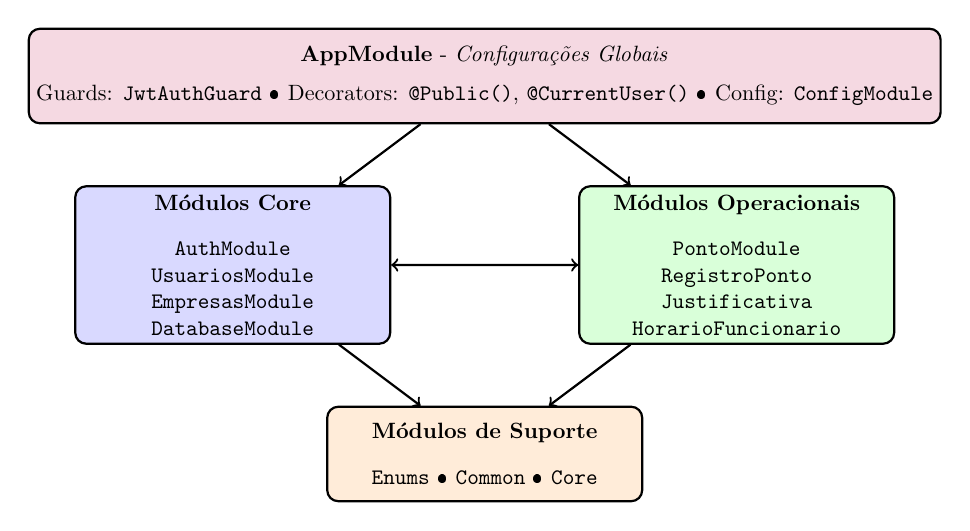
\begin{tikzpicture}[scale=0.8, every node/.style={transform shape}]
        % AppModule - Configurações Globais
        \node[draw, rounded corners, thick, fill=purple!15, minimum width=10cm, minimum height=1.5cm, align=center] (app) at (4,6) {
            \textbf{AppModule} - \textit{Configurações Globais}\\[0.2cm]
            Guards: \texttt{JwtAuthGuard} • Decorators: \texttt{@Public()}, \texttt{@CurrentUser()} • Config: \texttt{ConfigModule}
        };

        % Módulos Core
        \node[draw, rounded corners, thick, fill=blue!15, minimum width=5cm, minimum height=2.5cm, align=center] (core) at (0,3) {
            \textbf{Módulos Core}\\[0.3cm]
            \texttt{AuthModule}\\
            \texttt{UsuariosModule}\\
            \texttt{EmpresasModule}\\
            \texttt{DatabaseModule}
        };

        % Módulos Operacionais
        \node[draw, rounded corners, thick, fill=green!15, minimum width=5cm, minimum height=2.5cm, align=center] (operational) at (8,3) {
            \textbf{Módulos Operacionais}\\[0.3cm]
            \texttt{PontoModule}\\
            \texttt{RegistroPonto}\\
            \texttt{Justificativa}\\
            \texttt{HorarioFuncionario}
        };

        % Módulos de Suporte
        \node[draw, rounded corners, thick, fill=orange!15, minimum width=5cm, minimum height=1.5cm, align=center] (support) at (4,0) {
            \textbf{Módulos de Suporte}\\[0.3cm]
            \texttt{Enums} • \texttt{Common} • \texttt{Core}
        };

        % Setas
        \draw[->, thick] (app) -- (core);
        \draw[->, thick] (app) -- (operational);
        \draw[<->, thick] (core) -- (operational);
        \draw[->, thick] (core) -- (support);
        \draw[->, thick] (operational) -- (support);
    \end{tikzpicture}
    \caption{Organização modular do backend do sistema de registro de ponto.}
    \label{fig:arquitetura-backend}
\end{figure}

Como demonstrado no diagrama, os módulos de negócio possuem interdependências explícitas. O \texttt{AuthModule}, por exemplo, depende do \texttt{UsuariosModule} para validar credenciais e gerar tokens. Similarmente, o \texttt{PontoModule} interage com o \texttt{UsuariosModule} para associar registros a funcionários e com o \texttt{EmpresasModule} para validar regras de geolocalização.

\subsection{Padrões de Projeto e Camadas Arquiteturais}

A arquitetura de cada módulo é rigorosamente organizada em camadas, seguindo as melhores práticas de separação de responsabilidades.

\begin{description}
    \item[Camada de Apresentação (Controllers)] Responsável por expor os \textit{endpoints} da API RESTful. Os \textit{controllers}, como o \texttt{PontoController}, utilizam \textit{decorators} do NestJS para mapear rotas HTTP e verbos (GET, POST, etc.). A validação e transformação dos dados de entrada (DTOs - \textit{Data Transfer Objects}) é realizada automaticamente pelos \textit{Pipes} do NestJS, integrados com as bibliotecas \texttt{class-validator} e \texttt{class-transformer}.

    \item[Camada de Negócio (Services)] Concentra toda a lógica de negócio da aplicação. Os \textit{services}, como o \texttt{PontoService}, são injetados nos \textit{controllers} e são responsáveis por orquestrar as operações, validar as regras de negócio — como a verificação de sequência de registros de ponto implementada no \texttt{PontoValidatorService} e interagir com a camada de acesso a dados.

    \item[Camada de Acesso a Dados (Repositories)] A interação com o banco de dados PostgreSQL é abstraída pelo TypeORM, que implementa o padrão de projeto \textit{Repository}. Cada entidade, como a \texttt{RegistroPonto}, possui um repositório correspondente, que é injetado nos \textit{services} para realizar as operações de persistência (CRUD).

    \item[Camada de Segurança (Guards)] A segurança dos \textit{endpoints} é garantida através dos \textit{Guards} do NestJS. O \texttt{JwtAuthGuard}, por exemplo, é aplicado globalmente para proteger todas as rotas, exceto aquelas marcadas com o decorador \texttt{@Public()}, garantindo que apenas usuários autenticados possam acessar os recursos.
\end{description}

\section{Arquitetura do Front-End}

A arquitetura da aplicação \textit{frontend} foi projetada para ser moderna, performática e manutenível, utilizando o \textit{framework} Next.js (versão 14) com React (versão 18). A escolha pelo Next.js se justifica por sua arquitetura híbrida, que permite a renderização tanto no lado do servidor (\textit{Server-Side Rendering} - SSR) quanto no lado do cliente (\textit{Client-Side Rendering} - CSR) através do App Router. Essa flexibilidade é crucial para otimizar o tempo de carregamento inicial (\textit{First Contentful Paint} - FCP) das páginas públicas e garantir a interatividade das páginas do \textit{dashboard} \cite{STRAPI2024}.

\subsection{Estrutura Organizacional e Fluxo de Dados}

A aplicação segue uma arquitetura baseada em componentes, onde a interface do usuário é decomposta em peças reutilizáveis e de responsabilidade única. A estrutura de diretórios e o fluxo de dados entre as diferentes camadas da aplicação estão ilustrados na Figura~\ref{fig:arquitetura-frontend}.

\begin{figure}[htbp]
    \centering
    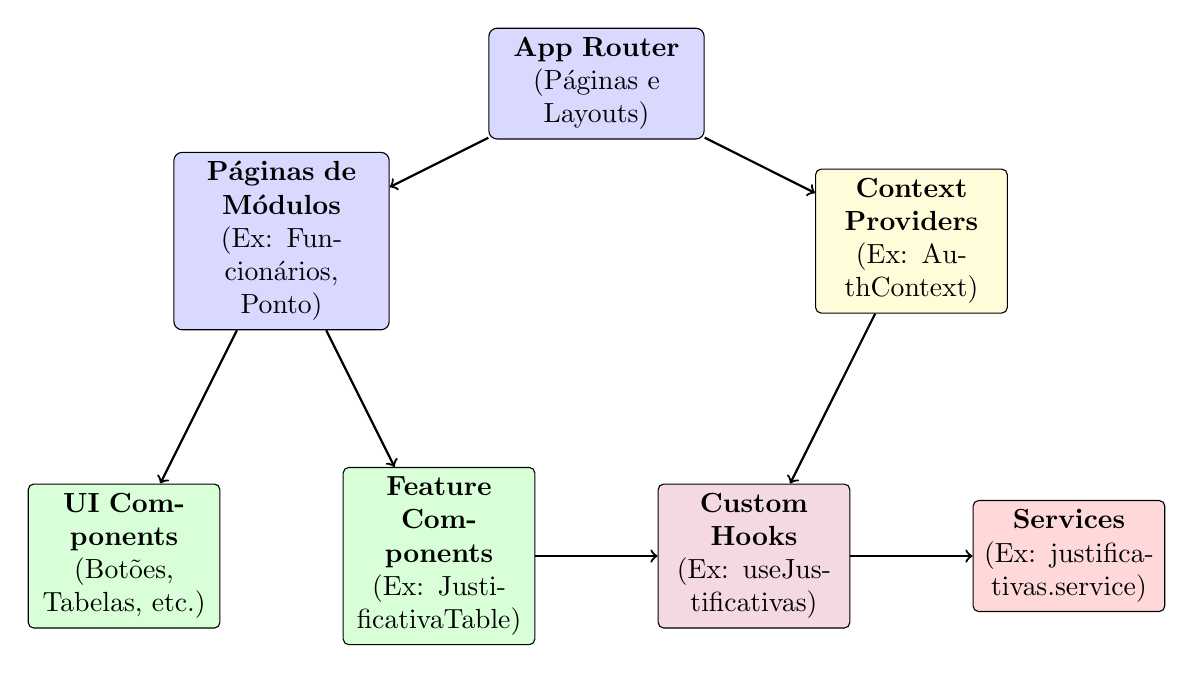
\begin{tikzpicture}[
            page/.style={rectangle, draw, fill=blue!15, text width=2.5cm, text centered, minimum height=1cm, rounded corners=3pt},
            component/.style={rectangle, draw, fill=green!15, text width=2.2cm, text centered, minimum height=1cm, rounded corners=2pt},
            context/.style={rectangle, draw, fill=yellow!15, text width=2.2cm, text centered, minimum height=1cm, rounded corners=2pt},
            service/.style={rectangle, draw, fill=red!15, text width=2.2cm, text centered, minimum height=1cm, rounded corners=2pt},
            hook/.style={rectangle, draw, fill=purple!15, text width=2.2cm, text centered, minimum height=1cm, rounded corners=2pt}
        ]

        % Nível 1: Roteamento e Layouts
        \node[page] (router) at (0,8) {\textbf{App Router}\\(Páginas e Layouts)};

        % Nível 2: Componentes de Alto Nível e Contextos
        \node[page] (pages) at (-4,6) {\textbf{Páginas de Módulos}\\(Ex: Funcionários, Ponto)};
        \node[context] (contexts) at (4,6) {\textbf{Context Providers}\\(Ex: AuthContext)};

        % Nível 3: Lógica e UI
        \node[component] (ui-comps) at (-6,2) {\textbf{UI Components}\\(Botões, Tabelas, etc.)};
        \node[component] (feature-comps) at (-2,2) {\textbf{Feature Components}\\(Ex: JustificativaTable)};
        \node[hook] (hooks) at (2,2) {\textbf{Custom Hooks}\\(Ex: useJustificativas)};
        \node[service] (services) at (6,2) {\textbf{Services}\\(Ex: justificativas.service)};

        % Conexões
        \draw[->, thick] (router) -- (pages);
        \draw[->, thick] (router) -- (contexts);
        \draw[->, thick] (pages) -- (ui-comps);
        \draw[->, thick] (pages) -- (feature-comps);
        \draw[->, thick] (feature-comps) -- (hooks);
        \draw[->, thick] (contexts) -- (hooks);
        \draw[->, thick] (hooks) -- (services);

    \end{tikzpicture}
    \caption{Fluxo de dados e arquitetura de componentes do frontend.}   \label{fig:arquitetura-frontend}     \end{figure}`

O fluxo de dados segue uma direção clara: o App Router renderiza as Páginas, que são compostas por Componentes de UI (elementos genéricos como botões e tabelas, localizados em src/components/ui) e Componentes de Funcionalidade (específicos de um domínio, como JustificativaTable). A lógica de estado e as chamadas de API são abstraídas em Hooks customizados e Services, que por sua vez consomem os Context Providers para acessar o estado global.

\subsection{Gerenciamento de Estado}

O gerenciamento de estado da aplicação adota uma abordagem híbrida, selecionando a ferramenta mais adequada para cada tipo de estado, conforme recomendado por padrões modernos de desenvolvimento React \cite{ReactDocsState}.

\begin{description}
    \item[Estado Local:] Para estados que pertencem a um único componente, como o controle de um modal ou o valor de um campo de texto, utiliza-se o \textit{hook} nativo do React, \texttt{useState}.
    \item[Estado Global Compartilhado:] Para estados que precisam ser compartilhados entre múltiplos componentes, como os dados do usuário autenticado, foi implementada a Context API do React. O \texttt{AuthContext}, por exemplo, provê as informações de autenticação para toda a árvore de componentes da aplicação.
    \item[Estado de Servidor (Server State):] A comunicação com a API, incluindo cache, revalidação e mutações de dados, é gerenciada pela biblioteca TanStack Query (React Query). Hooks customizados, como o \texttt{useJustificativas}, encapsulam a lógica do React Query, abstraindo as chamadas realizadas através dos \textit{services} e simplificando o uso nos componentes.
    \item[Estado de Formulários:] Para a gestão de formulários complexos, como o de cadastro de funcionários, foi adotada a biblioteca React Hook Form, que otimiza a performance ao evitar re-renderizações desnecessárias e simplifica a implementação de validações com a biblioteca Zod.
\end{description}

Essa estratégia de separação dos tipos de estado resulta em uma aplicação mais performática, organizada e com uma separação de responsabilidades bem definida.

\section{Fluxo de Autenticação e Autorização}

A segurança da aplicação é garantida por uma arquitetura integrada que combina a gestão de sessão no \textit{frontend} com a validação de tokens no \textit{backend}. O sistema implementa um fluxo de autenticação robusto baseado em JWT (\textit{JSON Web Tokens}), assegurando que todas as comunicações entre cliente e servidor sejam seguras e autorizadas. O diagrama de sequência na Figura~\ref{fig:fluxo-auth} ilustra o processo detalhado de login, desde a requisição do usuário até a geração do token de acesso.

\begin{figure}[htbp]
    \centering
    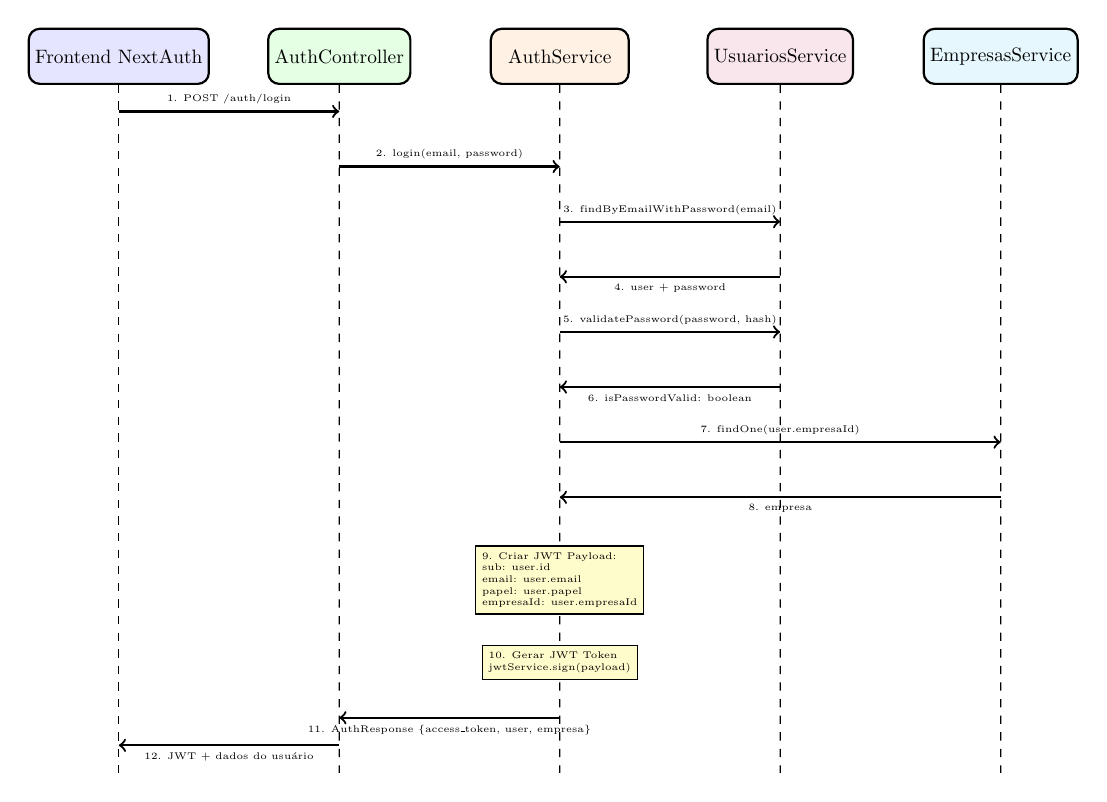
\begin{tikzpicture}[scale=0.7, every node/.style={transform shape}]
        % Participantes
        \node[draw, rounded corners, thick, fill=blue!10, minimum width=2.5cm, minimum height=1cm] (client) at (0,12) {Frontend NextAuth};
        \node[draw, rounded corners, thick, fill=green!10, minimum width=2.5cm, minimum height=1cm] (auth) at (4,12) {AuthController};
        \node[draw, rounded corners, thick, fill=orange!10, minimum width=2.5cm, minimum height=1cm] (service) at (8,12) {AuthService};
        \node[draw, rounded corners, thick, fill=purple!10, minimum width=2.5cm, minimum height=1cm] (users) at (12,12) {UsuariosService};
        \node[draw, rounded corners, thick, fill=cyan!10, minimum width=2.5cm, minimum height=1cm] (company) at (16,12) {EmpresasService};

        % Linhas de vida
        \draw[dashed] (client) -- (0,-1);
        \draw[dashed] (auth) -- (4,-1);
        \draw[dashed] (service) -- (8,-1);
        \draw[dashed] (users) -- (12,-1);
        \draw[dashed] (company) -- (16,-1);

        % Mensagens do fluxo de autenticação
        \draw[->, thick] (0,11) -- node[above, font=\tiny]{1. POST /auth/login} (4,11);
        \draw[->, thick] (4,10) -- node[above, font=\tiny]{2. login(email, password)} (8,10);
        \draw[->, thick] (8,9) -- node[above, font=\tiny]{3. findByEmailWithPassword(email)} (12,9);
        \draw[<-, thick] (8,8) -- node[below, font=\tiny]{4. user + password} (12,8);
        \draw[->, thick] (8,7) -- node[above, font=\tiny]{5. validatePassword(password, hash)} (12,7);
        \draw[<-, thick] (8,6) -- node[below, font=\tiny]{6. isPasswordValid: boolean} (12,6);
        \draw[->, thick] (8,5) -- node[above, font=\tiny]{7. findOne(user.empresaId)} (16,5);
        \draw[<-, thick] (8,4) -- node[below, font=\tiny]{8. empresa} (16,4);

        % Processamento interno no AuthService
        \node[draw, fill=yellow!20, align=left, font=\tiny] at (8,2.5) {9. Criar JWT Payload:\\sub: user.id\\email: user.email\\papel: user.papel\\empresaId: user.empresaId};

        \node[draw, fill=yellow!20, align=left, font=\tiny] at (8,1) {10. Gerar JWT Token\\jwtService.sign(payload)};

        \draw[<-, thick] (4,0) -- node[below, font=\tiny]{11. AuthResponse \{access\_token, user, empresa\}} (8,0);
        \draw[<-, thick] (0,-0.5) -- node[below, font=\tiny]{12. JWT + dados do usuário} (4,-0.5);
    \end{tikzpicture}
    \caption{Diagrama de sequência - fluxo de autenticação}
    \label{fig:fluxo-auth}
\end{figure}

\section{Fluxo de Autenticação e Segurança}

A segurança da aplicação é garantida por uma arquitetura integrada que combina a gestão de sessão no \textit{frontend} com a validação de tokens no \textit{backend}. O sistema implementa um fluxo de autenticação robusto baseado em JWT (\textit{JSON Web Tokens}), assegurando que todas as comunicações entre cliente e servidor sejam seguras e autorizadas. O diagrama de sequência na Figura~\ref{fig:fluxo-auth} ilustra o processo detalhado de login, desde a requisição do usuário até a geração do token de acesso.

\subsection{Arquitetura de Segurança}

A estratégia de segurança foi implementada através da orquestração de componentes especializados em cada camada da aplicação, que operam de forma coesa para proteger os dados e as funcionalidades do sistema.

No \textit{frontend}, a biblioteca NextAuth.js é responsável por gerenciar todo o ciclo de vida da sessão do usuário. Ela provê a interface de login, armazena o JWT recebido do \textit{backend} em um cookie HTTP-only seguro e gerencia os \textit{callbacks} de autenticação. Para proteger as rotas da aplicação, um Middleware (middleware.ts) intercepta as requisições de navegação, verifica a existência de uma sessão válida e redireciona usuários não autenticados para a página de login, garantindo que apenas usuários logados acessem o \textit{dashboard}.

No \textit{backend}, a segurança é implementada pelo \texttt{AuthModule}. A validação de cada requisição é feita por uma Estratégia JWT customizada (jwt.strategy.ts), que utiliza a biblioteca Passport.js para extrair e validar o \textit{payload} do token. A proteção dos \textit{endpoints} é aplicada através de Guards do NestJS. O \texttt{JwtAuthGuard} é implementado globalmente para proteger todas as rotas por padrão, enquanto um sistema de Controle de Acesso Baseado em Papéis (RBAC) permite a aplicação de restrições mais granulares, com níveis de acesso definidos como funcionário, administrador e proprietário.

\subsection{Validação de Geolocalização no Registro de Ponto}

Um dos diferenciais de segurança e conformidade do sistema é a validação de geolocalização para os registros de ponto, cuja lógica de negócio reside no \texttt{PontoService} do \textit{backend}. O processo é iniciado no \textit{frontend}, que utiliza a API de Geolocalização do navegador para capturar as coordenadas do dispositivo do funcionário no momento do registro.

Essas coordenadas são enviadas para a API, onde um algoritmo de validação executa os seguintes passos: recupera as coordenadas cadastradas da empresa; calcula a distância esférica entre os dois pontos utilizando a fórmula de Haversine, que considera a curvatura da Terra para maior precisão; e, por fim, verifica se a distância calculada está dentro do raio de tolerância configurado pela empresa. Registros fora do perímetro exigem obrigatororiamente uma justificativa do funcionário, garantindo a integridade e a rastreabilidade dos dados de ponto.